\documentclass{kulakarticle}
\usepackage{graphicx} % Required for inserting images
\usepackage[dutch]{babel}
\usepackage{amsmath}\usepackage{hyperref}
\usepackage{url}
\usepackage{float}
\title{Eindverslag: De slimme brandblusser}
\author{C. Callewaert, R. Nollet \\
	 C. Matvij, M. Van Insberghe, T. Wyckaert }
\date{Academiejaar 2022 -- 2023}
\address{
	\textbf{Groep Wetenschap \& Technologie Kulak} \\
	IW1 \\
	PnO}
\begin{document}
	
\maketitle

\tableofcontents

\pagebreak
 
\section*{Inleiding}

In het bedrijfsleven zijn er enorm veel wetten en regels om de veiligheid te optimaliseren. Brandveiligheid is hiervan een van de belangrijkste. Het aanwezig zijn van een automatisch brandblussysteem in een bedrijf is dan ook verplicht. Het populairste systeem is het sprinklersysteem. Deze heeft een groot bereik en kan grote gebouwen dus eenvoudig en efficiënt blussen. Het nadeel aan dit systeem is echter dat er veel installatie- en onderhoudskosten aan te pas komen. Daarom wordt een goedkoper alternatief gezocht zonder daarbij de brandveiligheid te verminderen. Het ontwerp van de "slimme" brandblusser komt hiervoor aan de pas. Deze brandblusser detecteert brand met behulp van een camera en kan automatisch een waterstraal richten op de brand en deze in een mum van tijd uitblussen. Om  de brandblusser op de markt te brengen, moet deze wel nog uitgebreid getest worden omdat het idee nog in zijn kinderschoenen staat. In dit artikel bespreken we het ontwerp, de bouw en de testresultaten van de slimme brandblusser. 


\section{Planning}

Omdat we bij dit project een deadline hebben gekregen, is het belangrijk om een goede planning te maken zodat we tijdig klaar geraken. Hiervoor hebben we gebruik gemaakt van een Gantt Chart. Dit is een \LaTeX-functie die toelaat om de deeltaken zorgvuldig weer te geven met de bijhorende deadlines. Zo kunnen we een goed overzicht bewaren over de actieve taken, hoelang er nog aan gewerkt zal worden etc. Op deze manier worden er geen taken dubbel gemaakt en blijven we op de hoogte van de voortgang van het project.  De taken van de Gantt Chart worden verdeeld onder de teamleden. Als een taak volbracht is, is het eenvoudig  te zien aan welke taak je vervolgens kan beginnen werken.

De belangrijkste taken zijn de mathematische berekeningen voor de waterstraal, de code voor de camera om de brand te herkennen, de interface om het apparaat te besturen en het tekenen van ons ontwerp. Het zijn deze taken die onderverdeeld worden in deeltaken en in de Gantt Chart gepland zijn. Eerst hebben we de klantenvereisten overlopen om te weten waaraan de brandblusser moet voldoen. Omdat we niet kunnen beginnen ontwerpen zonder te weten welk materiaal er te beschikking staat, is het logisch om hierna eerst te kijken wat er in de aanbieding staat. Om een idee te hebben over het ontwerp, is een eerste schets van de brandblusser nodig. Dit is al een behoorlijk accuraat ontwerp waaruit we kunnen afleiden welke materialen en software we zullen nodig hebben om ons idee te realiseren.  Hierna zal onder andere het programmeren en het tekenen van de nodige onderdelen, die we moeten 3D-printen, beginnen.

Omdat er waarschijnlijk nog wijzigingen zullen gebeuren, zal het printen zelf nog even op zich moeten laten wachten zodat we geen credits en materiaal verspillen. De mathematische berekeningen rond de ideale waterstraal en mondstuk zullen ook tijd vergen.  Ook moet onze camera geïnitialiseerd worden zodat deze rood herkent.  Omdat deze taken chaotisch door elkaar kunnen lopen,  zal ieder teamlid zich op een van deze taken focussen.  





\section{Ontwerpproces}
Van het moment dat we ons over dit project bogen hadden we allen al een sterke voorkeur om ons brandblusapparaat aan het plafond te bevestigen. Dit lijkt ons logischer aangezien er in een magazijn of werkplek vaak grote machines en hoge rekken staan die het zicht van onze camera beperken. Daarnaast legt onze waterstraal een korter traject af waardoor het minder last heeft van eventuele turbulenties. Deze slimme keuze levert ons een zo goed als perfect laminaire straal op die bijzonder voordelig is voor de dracht van ons water.

Ons oorspronkelijke idee was om een halve sfeer te 3D-printen die op een waterdichte houten bak bevestigd is die een motor, een tandwielkast, de voeding, de MyRio en de printplaten bevat. Op deze manier kunnen we zo veel mogelijk elektrische apparaten af te sluiten voor het water die uit onze jerrycan en pomp komt bij eventuele complicaties. In de sfeer is een inkeping voorzien voor de lans van onze brandslang. Om materiaal te besparen en de kosten te beperken hebben we uiteindelijk gekozen voor twee geprinte bogen die voorzien zijn van een kleine inkeping die het mondstuk stabiel houden (zie figuur \ref{figbompakanon_2}). Deze bogen zijn vervolgens bevestigd op een MDF-plaat waarin de nodige voorzieningen zijn gemaakt voor tandwielkasten, het mondstuk en de houder ervan. De brandblusser kan 90° roteren in horizontale richting en het mondstuk kan vrij roteren doorheen de twee beugels over een hoek van maximaal 90° met het plafond (zie figuur \ref{figZijAanzicht})

\begin{figure}[H]
	\centering
        \label{figbompakanon_2}
	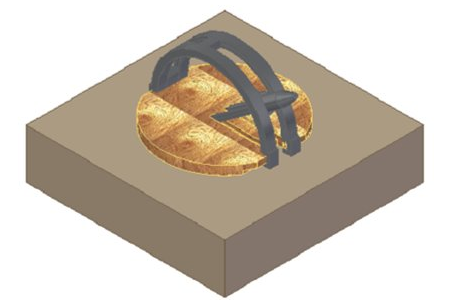
\includegraphics[width=0.6\textwidth]{Afbeeldingen/bompakanon.png}
        \caption{Totale Opstelling}
 
\end{figure}
\begin{figure}[H]
	\centering
        \label{figZijAanzicht}
	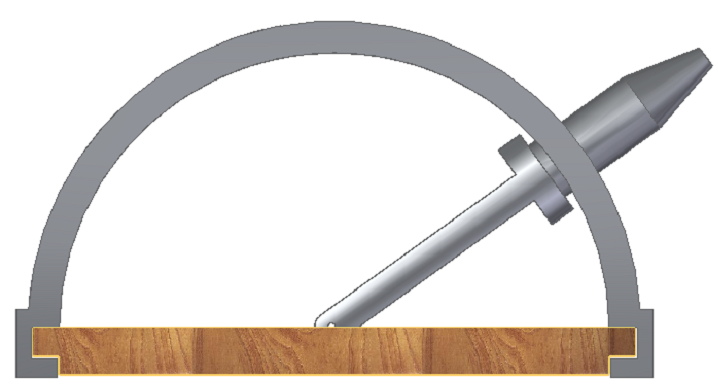
\includegraphics[width=0.6\textwidth]{Afbeeldingen/Screen_ZijAanzicht.png}
        \caption{zijaanzicht blusplatform}
 
\end{figure}

Hierna vestigden we onze aandacht op het ontwerp van het mondstuk. Ons eerste ontwerp bestond uit een opening voor de slang, een conische versmalling en een eindloop van 3mm. Berekeningen en extra opzoekwerk toonden daarna echter aan dat we beter af zouden zijn met een opening van 2mm en een complexer inwendig systeem. Dit inwendig systeem bestaat uit bijzonder veel kleine cilindrische gaten die de turbulente waterstroom uit de pomp zo laminair mogelijk maakt. Op die manier krijgen we meer water op de gewenste plaats en krijgen we een verhoging in ons bereik. Daarnaast zijn er onderaan horizontale cilindrische inkepingen gemaakt die voor voldoende wrijving zorgen met de waterslang zodat deze goed op zijn plek blijft zitten (zie figuur \ref{figmondstuk}).
\begin{figure}[H]
	\centering
        \label{figmondstuk}
	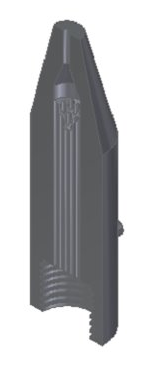
\includegraphics[width=0.15\textwidth]{Afbeeldingen/mondstuk.png}
        \caption{Mondstuk}
 
\end{figure}


\subsection{Hardware}
Als controller voor de motoren en pomp kozen we voor de MyRIO. 
MyRIO staat voor My Reconfigurable I/O, en is een krachtige en compacte microcontroller. De MyRIO ondersteunt heel wat connectiemogelijkheden. Men kan  verbinden met de MyRIO via WiFi of USB. Om met externe apparaten te communiceren ondersteunt de MyRIO heel wat communicatieprotocollen zoals I2C, SPI, UART etc. Ook kan de MyRio analoge waarden uitlezen en digitale toestellen aansturen. Voor onze toepassing moeten we enkele servo's aansturen. Dit wordt met een Pulse Width Modulation signaal(PMW) gedaan. De timing van dit signaal is van cruciaal belang voor de stabiliteit van de servo's. Om deze reden is de MyRIO ook een uitstekende keuze, het beschikt over hardware PWM die zeer nauwkeurig en stabiel is.\\
Voor de beweging van het mondstuk kozen we voor servomotoren. Deze motoren hebben ingebouwde encoders, waardoor de hoek heel nauwkeuring ingesteld kan worden. Alhoewel deze motoren slechts een beperkt draaibereik hebben zou dit voldoende moeten zijn voor onze toepassing. De servo's kunnen 17 kg-cm kracht leveren. We zullen binnenkort enkele tests uitvoeren om te controleren of deze motoren voldoende sterk zijn om het mondstuk en de slang te bewegen. \\
Als voeding gebruiken we de universele voeding van 12 volt voor de MyRIO en de pomp, en een step-down voltage regulator die de spanning naar 5 volt (of 6 volt) omvormt voor de servo's. 
De pomp sturen we aan met een relais die op zijn beurt door de MyRIO wordt aangestuurd.

\begin{figure}[H]
\begin{center}

    \label{fig:Schema}
    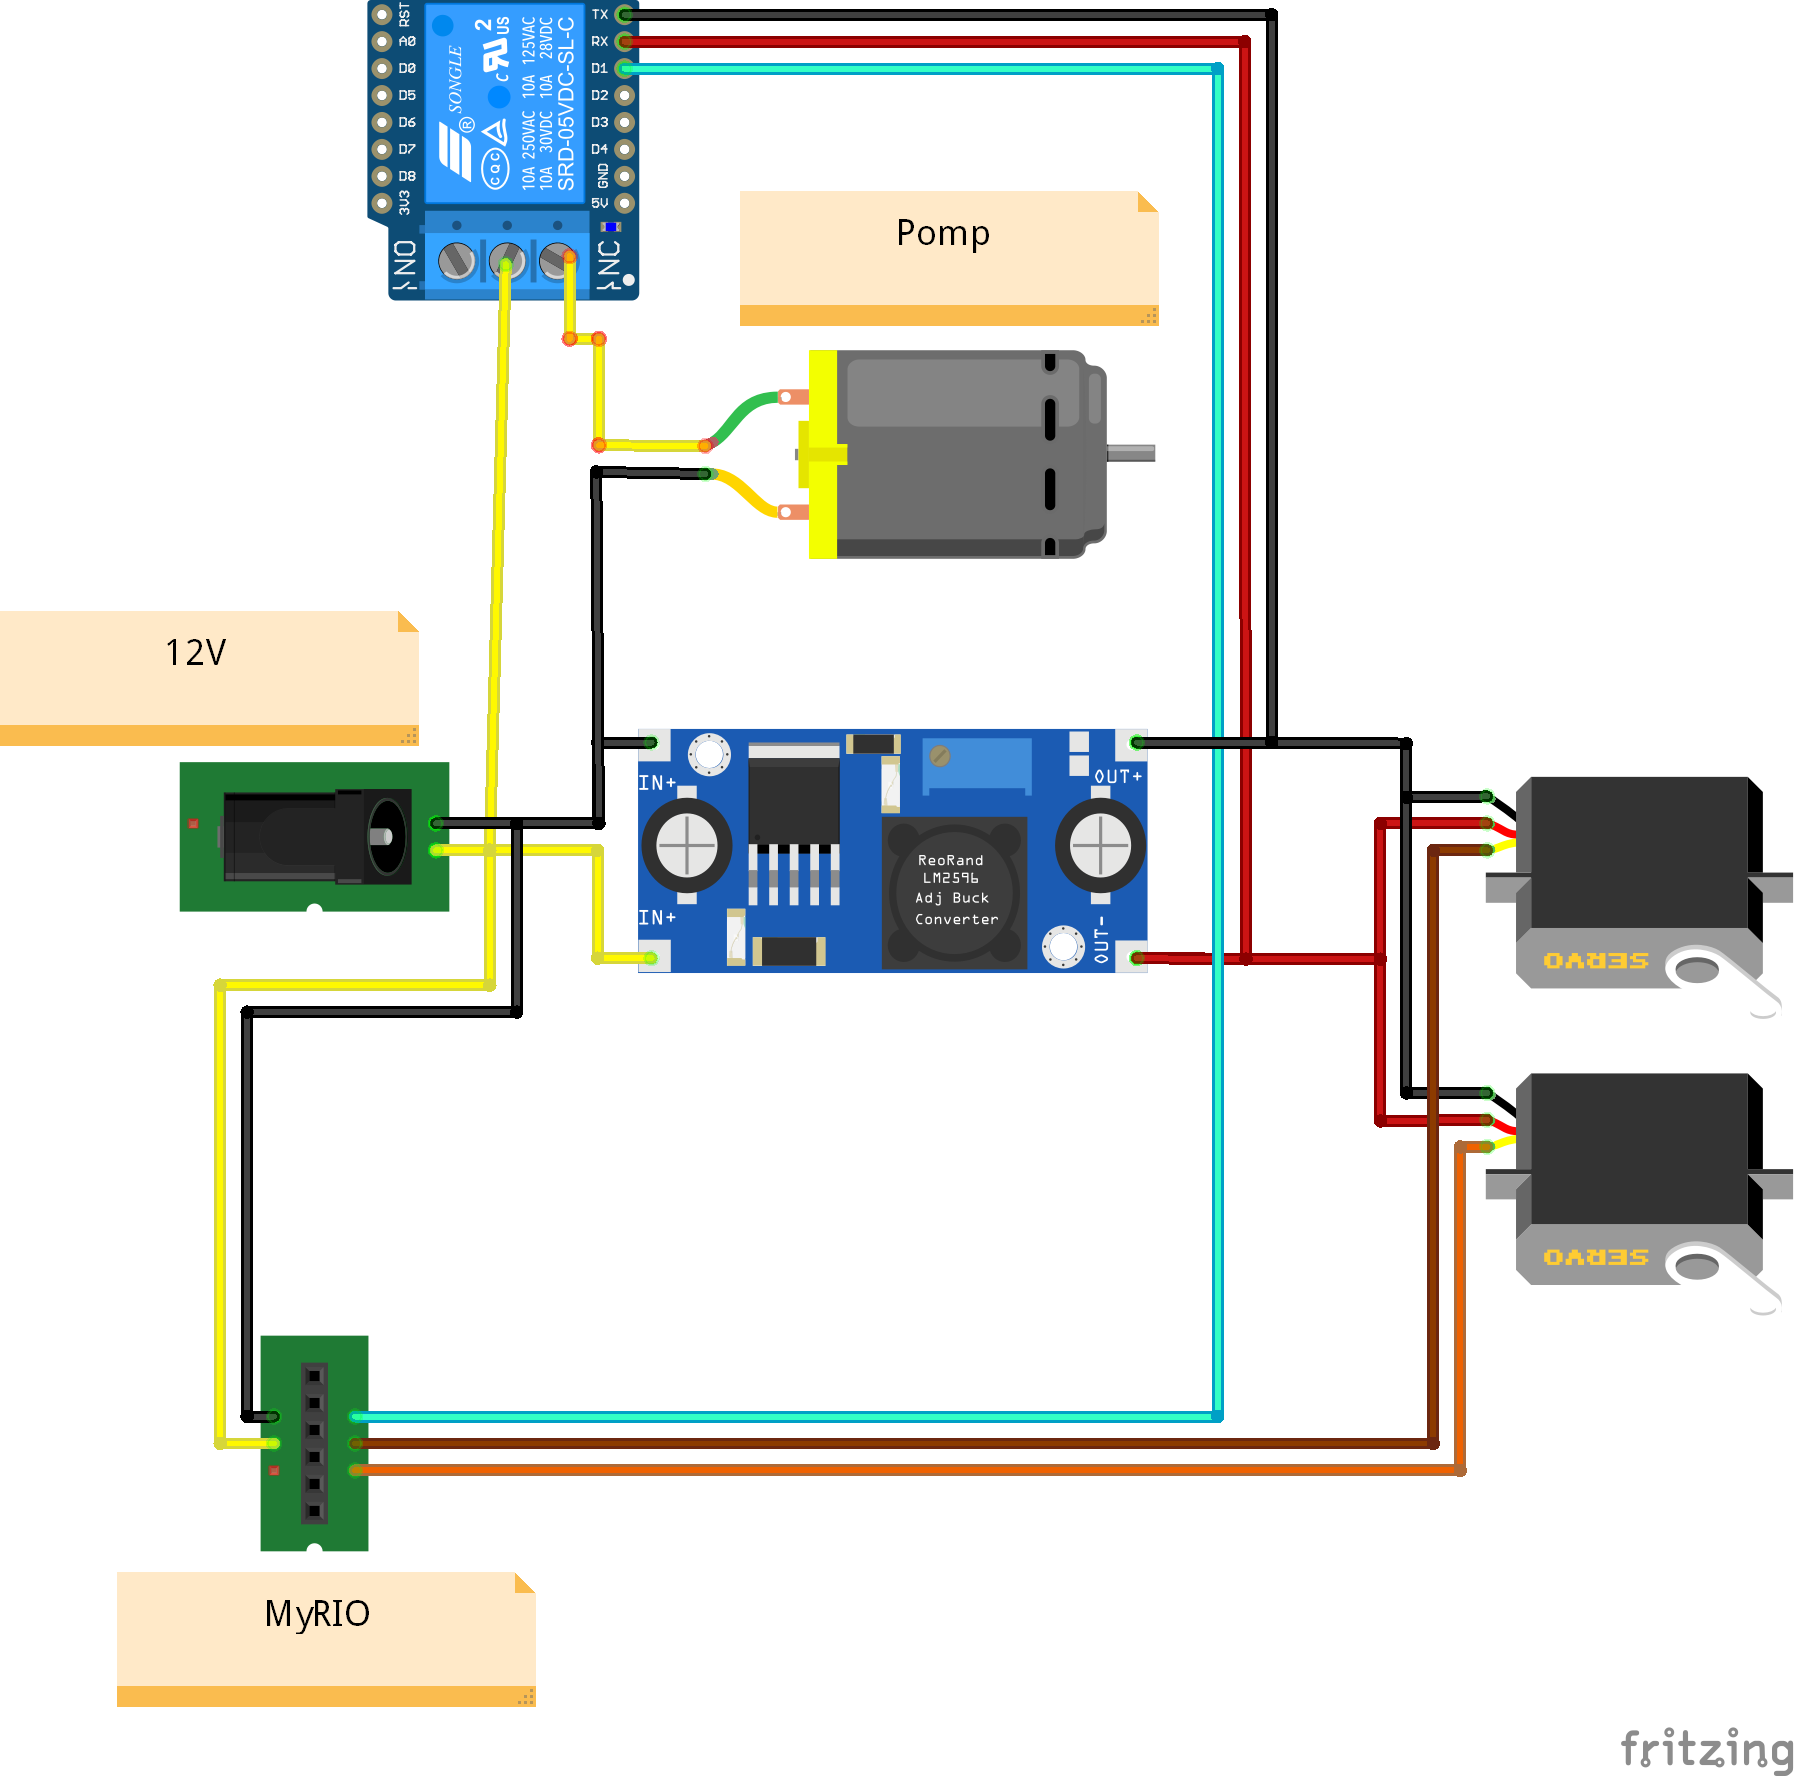
\includegraphics[width=0.5\textwidth]{Afbeeldingen/Schema.png}
    \caption{Elektrisch schema}

\end{center}
\end{figure}


\subsection{Software}
Ons programma wordt hoofdzakelijk geprogrammeerd in LabVIEW. Bepaalde onderdelen van de code worden echter geschreven in talen die voor specifieke toepassingen beter passen. Zo is de code  dat de objectdetectie uitvoert geschreven in Python omdat de OpenCV module zeer gebruiksvriendelijk is in dit progromama en er heel wat documentatie over te vinden is online. OpenCV staat voor Open Source Computer Vision Library. Dit is een open-source bibliotheek van algoritmen die vaak gebruikt wordt bij beeldverwerking. Een ander gedeelte wordt dan weer in Matlab geschreven, dat meer geschikt is voor wiskundige berekeningen. Al deze subprogramma's zullen we via LabVIEW integreren in het hoofdprogramma.\\
Het hoofdprogramma wordt op een computer uitgevoerd omdat de doelwitdetectie redelijk wat rekenkracht vergt. Dit programma staat ook in voor de manuele controle en de noodstop. Op de MyRIO zal een simpel programma staan dat de servo's en pomp kan aansturen aan de hand van commando's van het hoofdprogramma. Deze communiceren via een USB kabel. \\
Het hoofdprogramma detecteert eerst de locatie van de verschillende doelwitten door middel van een camera die met de computer verbonden is. Deze detectie gebeurt in een losstaande Python functie die de verschillende hoeken in de x-richting en afstanden in de y-richting van de doelwitten in een lijst teruggeeft. Vervolgens worden aan de hand van deze afstanden de hoek berekend in de y-richting, rekening houdend met de zwaartekracht en luchtweerstand op het water. Deze hoeken worden dan uiteindelijk naar de MyRIO gestuurd, die dan de servo's aanstuurt.

\subsection{Camera initialiseren}
Om de camera te programmeren zodat deze automatisch vuur (rode LEDs) herkent en de bijhorende coördinaten berekent, hebben we gebruik gemaakt van Python en OpenCV. 

Ons programma zet eerst het kleurbereik van de video input om van RGB (Red, Green, Blue) naar HSV (Hue, Saturation, Value). Op deze manier kunnen we een “mask” maken die filtert op alleen de felste pixels. In eerste instantie filterden we onze code op enkel rood licht, maar we ondervonden al snel dat dit een te groot bereik van kleuren was en dat de nauwkeurigheid niet echt optimaal was. Nu filteren we over een groter “Hue” bereik, maar enkel voor de allerhoogste “Value” (felste) waarden (zie figuur \ref{fig_saturation}) 


 \begin{figure}[H]
    \centering
    \label{fig_saturation}
	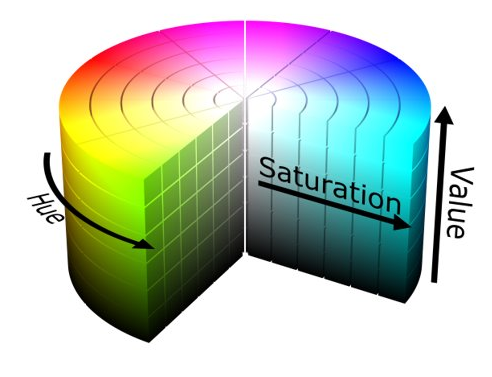
\includegraphics[width=0.6\textwidth]{Afbeeldingen/saturation.png}
    \caption{HSV kleurbereik}
 \end{figure}   




Nadat het programma de “mask” heeft gemaakt, gaat het op zoek naar de grootst mogelijke contouren die het kan vinden. Deze worden in een geordende lijst gezet. Daarna bepaalt het programma van de drie grootste contouren het middelpunt en trekt er een zo klein mogelijke cirkel rond. Met de straal van deze cirkel is het de bedoeling om er later de afstand  tot de objecten mee te bepalen. \ref{fig_focal}

\begin{figure}[h]
	\centering
        \label{fig_focal}
	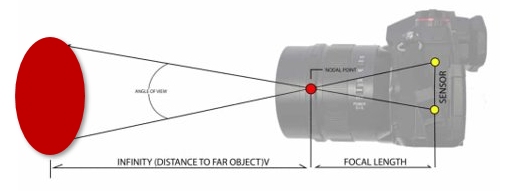
\includegraphics[width=0.6\textwidth]{Afbeeldingen/plaatsbepaling.png}
        \caption{plaatsbepaling brandpuntafstand}
 
\end{figure}

We zijn echter enkele onverwachte problemen tegengekomen waar we nog geen volledige oplossingen voor hebben weten te vinden. Het eerste probleem is het zicht van de camera. Na het bepalen van het horizontale en het verticale gezichtsveld van de camera, ondervonden we dat de camera niet het volledige veld in één keer kan zien. Het horizontaal gezichtsveld is normaal geen probleem, de camera ziet ongeveer 78° en we hebben slechts 75° nodig als we de camera op een van vooraf bepaalde hoogte van 2,5 m hangen. Het probleem zit hem in het verticaal gezichtsveld. Deze is slechts 18°, terwijl er zeker  26° nodig is. Een mogelijke oplossing hiervoor is het plaatsen van een extra servomotor zodat we de camera apart enkele graden kunnen draaien.

Een tweede probleem is de zogenaamde trapezium correctie. Doordat de camera niet loodrecht op het veld kijkt maar vanuit een hoek, kan deze niet zomaar de x-waarden vanop de video input aannemen als reële 3D x-waarden (zie figuur \ref{fig_trapezium}). Om de echte 3D waarden te bereken zullen we eerst een camera matrix moeten creëren met onder andere de brandpuntsafstand, het hoofdpunt en de hoek waarop de camera gemonteerd is. Verder moeten ook de vervormingscoëfficiënten van de camera bepaald worden. Wanneer deze matrix en coëfficiënten bepaald zijn kunnen we met behulp van enkele ingebouwde functies van openCV de 3D coördinaten bepalen. 

\begin{figure}[h]
	\centering
        \label{fig_trapezium}
	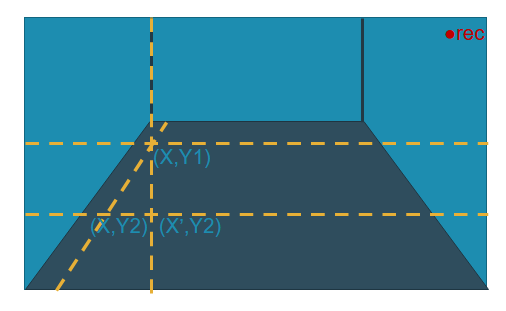
\includegraphics[width=0.6\textwidth]{Afbeeldingen/hoekprobleem.png}
        \caption{trapezium correctie}
 
\end{figure}

Met behulp van de 3D coördinaten berekent het programma uiteindelijk de graden waarop we het mondstuk moeten richten zodat de waterstraal tot aan de objecten raakt. Het programma houdt ook al rekening met de luchtweerstand en de divergentie van de waterstraal.


\subsection{Mathematische berekeningen}

In het proces van de bouw van de brandblusser is wiskunde een belangrijk onderdeel. Zo moeten  bijvoorbeeld de bewegingsvergelijkingen opgesteld worden, de waterstraalbanen moeten berekend worden net zoals de optimale hoek om dit te realiseren etc. 
Eerst en vooral werden verschillende manieren schriftelijk aangepakt. Zo werd de vrije val zonder weerstand eerst in het klad berekend om een algemeen idee te krijgen. Daarna werd deze met de kracht recht evenredig aan de snelheid bekeken, wat op eerste zicht een stuk makkelijker leek om op te lossen dan wanneer we met kwadratische snelheid rekenen. Als laatst werd  de meest accurate aanpak gebruikt waarbij de weerstandskracht recht evenredig is met de snelheid in het kwadraat. De laatste twee aanpakken bleken uiteindelijk hetzelfde probleem  te hebben. Beide moeten immers via trial and error de optimale hoek vinden met een gegeven gewenste afstand. 
Om de x- en y-coördinaten (afstand en hoogte respectievelijk) te plotten worden de vergelijkingen voor beide x en y opgesteld. Zo werd het volgende differentiaalstelsel bekomen: \newline


\(\frac{d}{dt}\) \begin{pmatrix}
 x\\
 y\\
 \dot{x}\\
 \dot{y}\\
\end{pmatrix}
= 
\begin{pmatrix}
\dot{x}\\
\dot{y}\\
-k\dot{x} \sqrt{\dot{x}^2+\dot{y}^2}\\
-g-k\dot{y} \sqrt{\dot{x}^2+\dot{y}^2}\\
\end{pmatrix} 
\newline
\newline
De x- en y-snelheid zijn afhankelijk van de initiële snelheid, die theoretisch afgeleidt werd uit het massadebiet van de pomp. Vanuit de berekeningen met behulp van de continuïteitsvergelijking wordt een zeer lage snelheid bekomen. Het mondstuk zal dus een smallere straal nodig hebben dan initïeel gedacht.
Via de functie ode45(ordinary differential equation) in Matlab kon dit stelsel makkelijk worden opgelost bij het meegeven van initiële waarden en de differentialen. De output is een matrix die de positie en snelheid van de x- en y-coördinaten en snelheden voor verschillende punten in een opgegeven tijdsspanne weergeeft. Om de optimale hoek te vinden werd voor elke baan de minimale afstand genomen tot het punt met x,y coördinaten (dist, 0), met 'dist' de gemeten afstand. Dit werd voor een 400-tal hoeken toegepast en al deze minima werden in een lijst gezet. Van deze lijst werd het minimum genomen waarvan de index werd onthouden, deze index zegt voor de hoeveelste hoek (iteratie) onze baan een minimale afstand heeft ten opzichte van het gewenste punt. Om de functie zo accuraat mogelijk de juiste hoek te laten kiezen, zal een zo groot mogelijk aantal hoeken nodig zijn en een zo groot mogelijk aantal geplotte punten. Ook moet rekening gehouden worden met de benodigde tijd van het programma. Na enkele testen uit te voeren bleek ca.400 hoeken met een tijdsspanne van 0-0.8s met intervallen van 0.005s na ca. 1s een output te maken. 
Ook zal deze functie een plot maken met de optimale waterstraalbaan en het snijpunt met de x-as en y-as die als x-component de ingegeven gewenste afstand geeft (zie figuur \ref{fig_optimalehoekplot}. 
\begin{figure}[H]
	\centering
        \label{fig_optimalehoekplot}
	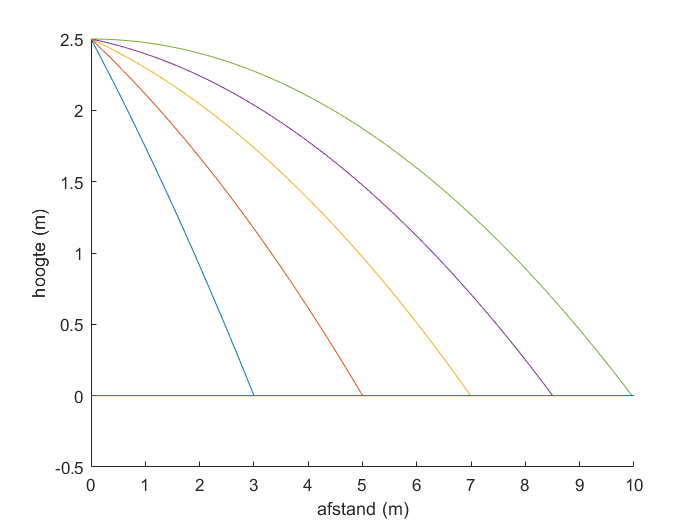
\includegraphics[width=0.6\textwidth]{Afbeeldingen/Waterstraalplot.png}
        \caption{Optimale hoek plot}

 
\end{figure}


Er zal zeer waarschijnlijk nog een afwijking zijn met de realiteit dus er zal nog geëxperimenteerd moeten worden om de in werkelijkheid initiële snelheid en de 'drag-coefficient' te bepalen.

\section*{Besluit}

Ons project is al goed gevorderd dus we zitten momenteel goed op schema. Ons ontwerp heeft op alle vlakken al een goede vordering gemaakt. We hebben ons materiaal en onze onderdelen al gekozen. Onze camera herkent ook al kleur en het 3D ontwerp van het blusplatform en het mondstuk zijn afgewerkt. Ook de mathematische functie voor de algemene hoek te vinden is ook al opgesteld. Wel hebben we nog theoretische uitkomsten die vermoedelijk niet kloppen met de praktijk.
Aan de assemblage moeten we wel nog beginnen. Dit zal na de paasvakantie gebeuren.
We hebben echter momenteel nog te maken met enkele problemen die we nog de nodige aandacht zullen moeten geven. Ons ontwerp is dus nog in volle ontwikkeling en zal nog enkele veranderingen ondergaan. Dit geldt vooral voor onze camera problemen. Ook zijn er nog enkele andere vraagtekens, onder andere de werkelijke initiële snelheid, de weerstandscoëfficient, het bereik van de straal en hoe laminair de stroom is. 

\newline
%\section*{bronnen}
%https://website.nbn.be/themas/brandveiligheid 
%https://en.wikipedia.org/wiki/Projectile\_motion
%https://docs.opencv.org/
%https://www.ni.com/nl-be/support

\clearpage
\nocite{*}
\bibliographystyle{unsrt}
\bibliography{referenties}





% nog de bronnenlijst
 %\printbibliography


\end{document}





   